%% Adaptado de
%% http://www.ctan.org/tex-archive/macros/latex/contrib/IEEEtran/
%% Traduzido para o congresso de IC da USP

\documentclass[twoside,conference,a4paper]{IEEEtran}


\usepackage{IEEEtsup} 
\usepackage[english,brazilian,brazil]{babel}
\usepackage[utf8]{inputenc}
\usepackage[T1]{fontenc}
\usepackage{latexsym,amsfonts,amssymb}
\usepackage{theorem}
\usepackage[cmex10]{amsmath} 
\usepackage{url}
\usepackage{graphicx}
\usepackage{amsmath}
\usepackage{amssymb}
\usepackage{color}
\usepackage[pagebackref=true,breaklinks=true,letterpaper=true,colorlinks,bookmarks=false]{hyperref}
\usepackage[tight,footnotesize]{subfigure}
\usepackage[noadjust]{cite}

\begin{document}
\selectlanguage{brazil}
\renewcommand{\IEEEkeywordsname}{Palavras-chave}

\urlstyle{tt}
\title{Reconhecimento de Imagens usando NAO e Redes Neurais}
\author{
 \IEEEauthorblockN{Jonatan  Tiago de  Souza Valongo\,\IEEEauthorrefmark{1}}
 \IEEEauthorblockA{\IEEEauthorrefmark{1}
                   Graduação, RA: 117424}\\

 \IEEEauthorblockN{Mariane Previde\,\IEEEauthorrefmark{1}}
 \IEEEauthorblockA{\IEEEauthorrefmark{1}
                   Graduação, RA: 121191}\\

 \IEEEauthorblockN{Rafael Timbó Matos\,\IEEEauthorrefmark{1}}
 \IEEEauthorblockA{\IEEEauthorrefmark{1}
                 Graduação, RA: 106228}\\

 \IEEEauthorblockN{Roberto Kasuho Hayasida Junior\,\IEEEauthorrefmark{1}}
 \IEEEauthorblockA{\IEEEauthorrefmark{1}
                 Aluno Especial, RA: 103984}\\
}


\maketitle

\begin{abstract}
 Este é um trabalho final de curso, da matéria Introdução à Inteligência Artificial, ministrada no primeiro semestre de 2016, na Universidade Estadual de Campinas, pela Professora Esther Luna Colombini. O objetivo desse trabalho é aplicar técnicas de IA vistas no decorrer do curso, utilizando o simulador V-REP e o robô NAO. O problema escolhido pelo grupo foi o de reconhecimento de imagens, obtidas através das câmeras do NAO. Mais especificamente, identificar se o objeto retratado é uma planta ou não. Para tal, utilizamos redes neurais artificiais.
\end{abstract}

\begin{IEEEkeywords}
 Inteligência artificial, redes neurais, reconhecimento de imagens, NAO, V-REP
\end{IEEEkeywords}


\section{Introdução}
Nesse trabalho buscamos aplicar as técnicas vistas em sala de aula, relacionadas a redes neurais, utilizando o simulador V-REP. Nas simulações, incluímos o robô NAO, que será o agente principal do cenário. O problema escolhido foi o de reconhecimento de imagens. Como o NAO possui em seu conjunto de sensores câmeras, decidimos utilizar as imagens obtidas por elas como input de uma rede neural cujo objetivo é determinar se a imagem retrata uma planta ou não. 
O campo de pesquisa de reconhecimento de padrões é de vasta aplicação prática, permeando diversos contextos da vida moderna, com utilização na indústria e em tecnologia pessoal. Um exemplo é o reconhecimento de faces em imagens publicadas por usuários de redes sociais. Outras aplicações, como reconhecimento de pedestres em imagens de câmeras de segurança ou a extração de textos de imagens (OCR), tornam-se cada vez mais comuns. Existem vários métodos e estratégias para esse problema, como utilização de modelos, de exemplos, técnicas baseadas em detecção de bordas, comparação de cores e gradientes, entre outras.
O NAO pode utilizar deste métodos para interagir com os objetos ao seu redor, como cumprimentar pessoas ou recolher objetos

\section{Redes Neurais Artificiais}
Redes Neurais Artificiais tem como inspiração os neurônios biológicos e tentam modelar matematicamente o seu comportamento.
Partindo de uma representação simples do neurônio, monta-se redes multi-camadas, formadas geralmente por uma cadama de entrada, camadas intermediárias ocultas e uma camada de saída. Os diversos componentes dessa redes estão interconectados e essas conexões tem pesos. O funcionamento básico de cada unidade pode ser descrito da seguinte forma:
\begin{enumerate}
 \item são fornecidos os valores de entrada;
 \item cada entrada tem seu valor multiplicado pelo peso de sua conexão;
 \item se a soma ponderada dessas multiplicações ultrapassar um limiar (threshold), a unidade produz um determinado valor de saída.
\end{enumerate}

A adaptação desses pesos é o que provê capacidade de aprendizado a uma rede.
Após treinamento, o conhecimento fica representado nesses valores dos pesos da rede. Para esta tarefa são necessários dois itens: um conjunto de treinamento e um algoritmo de aprendizado. O primeiro é um conjunto de elementos que servirão de exemplos e o algortimo de aprendizado determina como os pesos da conexões serão atualizados. É importante notar que os pesos são atualizado de acordo com uma taxa de aprendizado. Ela determina a influência da distância entre a saída esperada e obtida na atualizações dos pesos. Grandes taxas de aprendizados permitem atingir valores próximos do esperado com menos iterações, entretanto podem não convergir para a solução exata por possuir um passo muito grande.

Por outro lado, taxas de aprendizado menores costumam levar muito mais iterações para se aproximar do valor desejado, mas possuem uma granularidade melhor na busca da solução. Existem três paradigmas para esse aprendizado (supervisionado, não-supervisionado e reforço). No aprendizado supervisionado, utilizado neste projeto, possuimos um conjunto de treinamento cuja saída é conhecida. Assim, podemos alimentar a rede com a entrada do problema e averiguar a resposta da rede neural, corrigindo-a conforme necessário. A saída fornecida pela rede e a saída esperada são usados da seguinte forma:
\begin{itemize}
\item os pesos das conexões são iniciados com valores aleatórios
\item até que um critério de parada seja atingido (como um valor mínimo de erro ou fim do conjunto de exemplos), para cada elemento do conjunto de exemplo:
  \begin{itemize}
    \item a saída é calculada
    \item atualizam-se os pesos da conexões baseando-se na distância entre a saída obtida e a esperada
  \end{itemize}
\end{itemize}

Em relação a topologia das redes neurais, quando temos apenas uma só camada, os valores da entrada são mapeados diretamente em uma saída, e a eficiência da rede limita-se a contextos em que os padrões de entrada são suficientes para o mapeamento da solução. No caso de redes multi-camadas, as camadas ocultas intermediárias são conhecidas como extratoras de características. Elas permitem que a rede crie uma representação mais complexa do universo do problema. Nesse cenário, utiliza-se a retropropagação do erro para a atualização dos pesos das camadas internas.

Conforme a rede neural cresce, o processo se torna mais complexo, e requer mais iterações, uma das limitações dessa técnica. Redes grandes exigem um maior conjunto de entrada que represente a complexidade e diversidade do problema, para que a rede possa abstrair o padrão e aprender sobre o problema. Isto nos leva à outra limitação: nåo é possível extrair conhecimento de uma rede treinada-ela age como uma caixa preta. Assim, um desafio é encontrar o tamanho adequado da rede para o problema: a rede não deve ser complexa demais para o problema, causando gastos de recursos desnecessários, como também não deve ser excessivamente simples e incapaz de abstrair o conhecimento necessário para a resolução do problema. \cite{Colombini:2016} \cite{Carvalho:2016} \cite{Shiffman:2012}

\section{Projeto}
\subsection{Cenário}
\begin{figure}[ht]
\centering
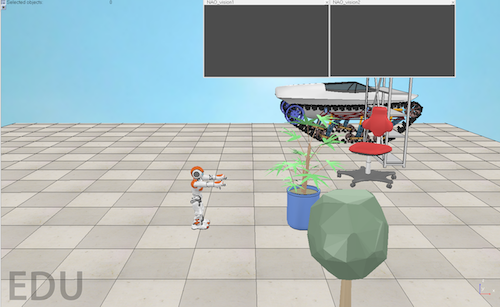
\includegraphics[width=1\hsize]{figuras/cenario1.png}
\caption{Cenário do simulador.}
\label{fig:fig1}
\end{figure}

De posse de um algoritmo capaz de reconhecer uma planta utilizando-se redes neurais, podemos conectá-lo ao robo NAO. Entretanto, diante da ausência deste, utilizamos o V-REP, uma plataforma de simulação virtual capaz de emular um NAO. Esta plataforma possui uma API com chamada remota em Python, onde podemos executar o nosso programa. 

O cenário utilizado no simulador é composto pelo robô NAO e objetos cujas imagens serão capturadas pelas câmeras do NAO. A planta fornecida pelo simulador foi utilizada como referência. Como referências não-planta utilizamos outros objetos do simulador. Como o problema está focado nos dados obtidos pelas câmeras, não precisamos nos preocupar com a locomoção do NAO.

Nosso algoritmo pode ser resumido em:
\begin{enumerate}
\item Carregar uma rede neural previamente salva em arquivo ou construí-la.
\item Treinar a rede com o conjunto de treinamento do banco de dados, se necessário
\item Salvar a rede em arquivo, se necessário
\item Conectar-se ao simulador e ao NAO
\item Loop:
  \begin{enumerate}
    \item Capturar imagem do sensor do NAO
    \item Alimentar a rede com a imagem obtida
    \item A rede responde indicando se a imagem contém uma planta ou não
  \end{enumerate}
\end{enumerate}

Podemos simular a movimentação do NAO simplesmente arrastando-o pelo cenário com o mouse, e o programa continuará recebendo as imagens do sensor e classificando a imagem apropriadamente.

\subsection{Implementação}
A rede neural, seus componentes e a aplicação cliente do simulador foram desenvolvidas utilizando Python, pois o simulador oferece ótimo suporte a esta linguagem, além de ser uma linguagem de alto nível com bibliotecas prontas para manipulação de imagens. As imagens foram obtidas a partir da API fornecida pelo simulador. A implementação da rede neural seguiu os seguintes parâmetros:
\begin{itemize}
\item Camadas: uma de entrada, uma intermediária e uma de saída;
\item Taxa de aprendizado: 0.1;
\item Entrada: imagens obtidas pelas câmeras;
\item Pesos iniciais: aleatórios;
\item Utilização de retropropagação dos erros.
\item Conjunto de treinamento: inicialmente composto por 35 imagens, dentre elas 17 com o objeto planta.
\end{itemize}

A escolha dessa topologia foi feita baseada no fato de o conjunto de treinamento ser limitado, assim como o escopo do problema (planta/não-planta). 

\subsection{Desenvolvimento, Evolução e Limitações}
Durante o desenvolvimento do projeto encontramos diversas limitações e dificuldades. Além de dificuldades técnicas com a linguagem e a API do simulador, a principal dificuldade foi ajustar a topologia da rede e o conjunto de treinamento.

Iniciamos considerando as imagens em escala de cinza, no tamanho padrão exportado pelo simulador (640x480), como um teste, com a intenção de evoluir para o uso de RGB. Nosso parâmetro inicial de iterações de treinamento foi 1000. Logo nessa primeira instância, foi possível perceber que esse número de iterações não seria viável, e então o reduzimos para 10. Porém a rede não foi capaz de chegar a uma solução. Ao tentarmos utilizar imagens coloridas, nos deparamos com uma outra limitação computacional: uma imagem na resolução que utilizávamos tem cerca de 300 mil pixels. Enquanto utilizávamos escalas de cinza, cada pixel representava uma entrada. Porém, se migrássemos para RGB, esse tamanho de entrada seria multiplicado por três. Não foi possível concluir esse cenário pois a aplicação exigiu mais memória do que tínhamos disponível. Descobriu-se também
que a linguagem Python pode consumir mais memória do que o necessário por causa de suas abstrações, frequentemente com bibliotecas implementadas em C para estrutura de dados e algoritmos cujos recursos são escassos.

\begin{figure}[ht]
\centering
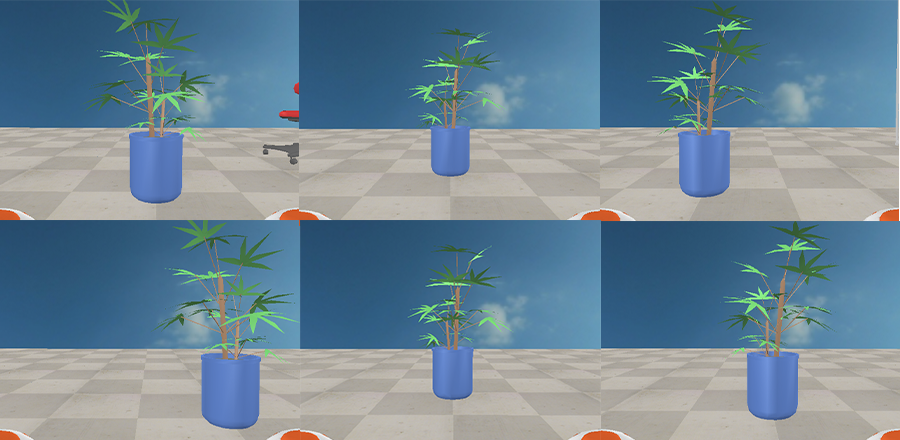
\includegraphics[width=1\hsize]{figuras/exemploconj1.png}
\caption{Exemplos de imagens de plantas do conjunto de treinamento inicial.}
\label{fig:fig2}
\end{figure}

Consideramos então reduzir o tamanho da imagem de entrada. Para não perdermos detalhes reduzindo a imagem como um todo, optamos por descartar as bordas laterais e focar no retângulo 320x480 central e por continuar a utilizar escala de cinza. Esse cenário mostrou-se viável computacionalmente, porém, novamente, não conseguimos chegar em uma solução. Em última instância, motivados pela topologia simples da rede e recursos computacionais limitados, optamos por aumentar a consistência do conjunto de treinamento, especificamente das imagens que teriam saída positiva.

Anteriormente, utilizamos imagens de plantas em diversas posições dentro do quadro e distâncias da câmera [Fig. \ref{fig:fig2}], assumindo que a rede seria capaz de abstrair o conceito de escala e posicionamento do objeto. Entretanto, isto se provou complexo para o escopo deste projeto e reduzimos esse subconjunto para apenas imagens da planta fixa em uma distância e enquadramento, rotacionado-a apenas em torno de seu próprio eixo [Fig. \ref{fig:fig3}]. A literatura sugere a adição de um fator de escala e posicionamento para lidar com as variações de distância do objeto à câmera e posicionamento deste no escopo de visão.

\begin{figure}[ht]
\centering
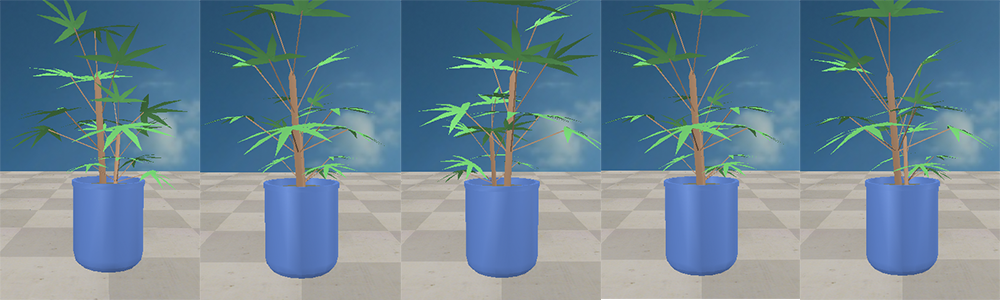
\includegraphics[width=1\hsize]{figuras/exemploconj2.png}
\caption{Exemplos de imagens de plantas do aegundo conjunto de treinamento.}
\label{fig:fig3}
\end{figure}

\section{Resultados e Conclusões}
Mesmo após diversos ajustes nos parâmetros da aplicação, não conseguimos chegar a uma solução. Apontamos como principais obstáculos dificuldades na implementação da rede neural e limitações computacionais que não permitiram que a topologia da rede fosse evoluída.

Com as experências obtidas durante o projeto, foi possível observar a complexidade das técnicas envolvidas no desenvolvimento de redes neurais, assim como a importância de boas definições do problema e seu universo, de um bom conjunto de treinamento e de iterações de ajustes até que se encontre uma boa topologia de rede para o problema.

 +-------------+

\bibliographystyle{IEEEtran}

\bibliography{Relatorio}

\end{document}
